\documentclass[conference]{IEEEtran}

\usepackage{amsmath}
\usepackage{graphicx}
\usepackage{booktabs}
\usepackage{array}
\usepackage{subcaption}
\usepackage{url}

% Upload these generated files from Model Simulation/ to Overleaf with this .tex:
% aeris_dual_objective_snapshots.png
% aeris_dual_objective_metrics.png
% benchmark_dual_on_5seed.png
% benchmark_watch_off_5seed.png
% benchmark_watch_guarded_on_5seed.png

\title{AERIS Project Update: Greedy Optimization Proof-of-Concept and Path Toward Receding-Horizon Control}

\author{
\IEEEauthorblockN{Jeewoo Choi}
\IEEEauthorblockA{
Stanford University\\
jchoi23@stanford.edu
}
}

\begin{document}
\maketitle

\begin{abstract}
AERIS studies autonomous UAV role allocation for resilient intelligence,
surveillance, and reconnaissance (ISR) in contested environments. The original
proposal framed the project as a graph-based optimization problem in which UAVs
must dynamically balance sensing, relay placement, energy, and connectivity to
the base station. Since the proposal, the project has progressed from a visual
simulation into a measurable benchmark environment with connected ISR scoring,
enemy detection latency, adaptive relay branching, dual-objective scenarios,
and multi-seed evaluation. The current controller is intentionally simple: it is
a greedy heuristic optimizer that demonstrates the feasibility of autonomous
role switching and relay-supported ISR. The final project phase will replace or
augment this heuristic with more robust optimization strategies, especially a
finite-horizon assignment optimizer that evaluates candidate UAV actions using a
multiobjective mission score.
\end{abstract}

\section{Original Project Objective}
The AERIS concept is based on the observation that ISR coverage is only useful
when the collected data can be transmitted back to the operator. A UAV that sees
an enemy but is disconnected from the base station does not provide valid
mission value. Therefore, the UAV team must jointly optimize two coupled goals:
collect useful ISR data and maintain a connected communication path.

The proposed UAV roles are:
\begin{itemize}
    \item \textbf{ISR Mode}: move to observe enemies or objectives.
    \item \textbf{Mobile Relay Mode}: move to preserve or repair network links.
    \item \textbf{Static Relay Mode}: hold position as a stronger communication node.
\end{itemize}

The original optimization objective can be summarized as:
\begin{equation}
\max \; w_1 C_{\text{ISR}}(t) + w_2 C_{\text{conn}}(t)
- w_3 E(t) - w_4 W_{\text{op}}(t) - w_5 N_{\text{switch}}(t),
\end{equation}
where $C_{\text{ISR}}$ is valid connected ISR coverage, $C_{\text{conn}}$ is
network connectivity, $E$ is energy use, $W_{\text{op}}$ is operator workload,
and $N_{\text{switch}}$ penalizes excessive role switching.

\section{Work Completed So Far}

\subsection{Simulation Environment}
The current project implements a discrete-time UAV simulation. At each timestep,
the simulator updates UAV motion, battery state, enemy motion, communication
links, connected components, ISR coverage, strike progress, objective health,
and policy decisions. This provides the foundation for evaluating UAV autonomy
policies under repeatable conditions.

\subsection{Connectivity-Constrained ISR Scoring}
The project now enforces the key constraint from the proposal: ISR observations
only count if the observing UAV is connected to the base station through the
communication graph. This turns the simulation from a simple visual tracker into
a mission-relevant graph problem.

\subsection{UAV Role Switching and Recovery Behavior}
UAVs can now switch among ISR, mobile relay, static relay, return-to-base, and
recharge states. The controller promotes ISR UAVs into relay roles when the
network requires additional communication support. Mobile relays can become
static relays after reaching useful waypoints, and low-battery UAVs return to
base before redeploying.

\subsection{Honest Mission Metrics}
The simulator now records per-enemy detection and observation history, including
spawn time, first detection time, alive time, and observed time. This supports
metrics such as:
\begin{itemize}
    \item time-weighted ISR coverage,
    \item average detection latency,
    \item north, center, and south flank coverage,
    \item connected UAV fraction,
    \item UAV losses,
    \item strikes completed,
    \item secondary objective health.
\end{itemize}
These metrics are more diagnostic than a single visual score because they reveal
whether the policy detects threats early or only appears successful after enemy
attrition.

\subsection{Dual-Objective Scenario}
A new scenario adds undefended north and south objectives. Enemies in the upper
and lower regions of the map move toward these objectives and damage them if
not detected and suppressed. This makes the problem more two-dimensional and
exposes the limitations of a single centerline relay chain.

\begin{figure*}[t]
    \centering
    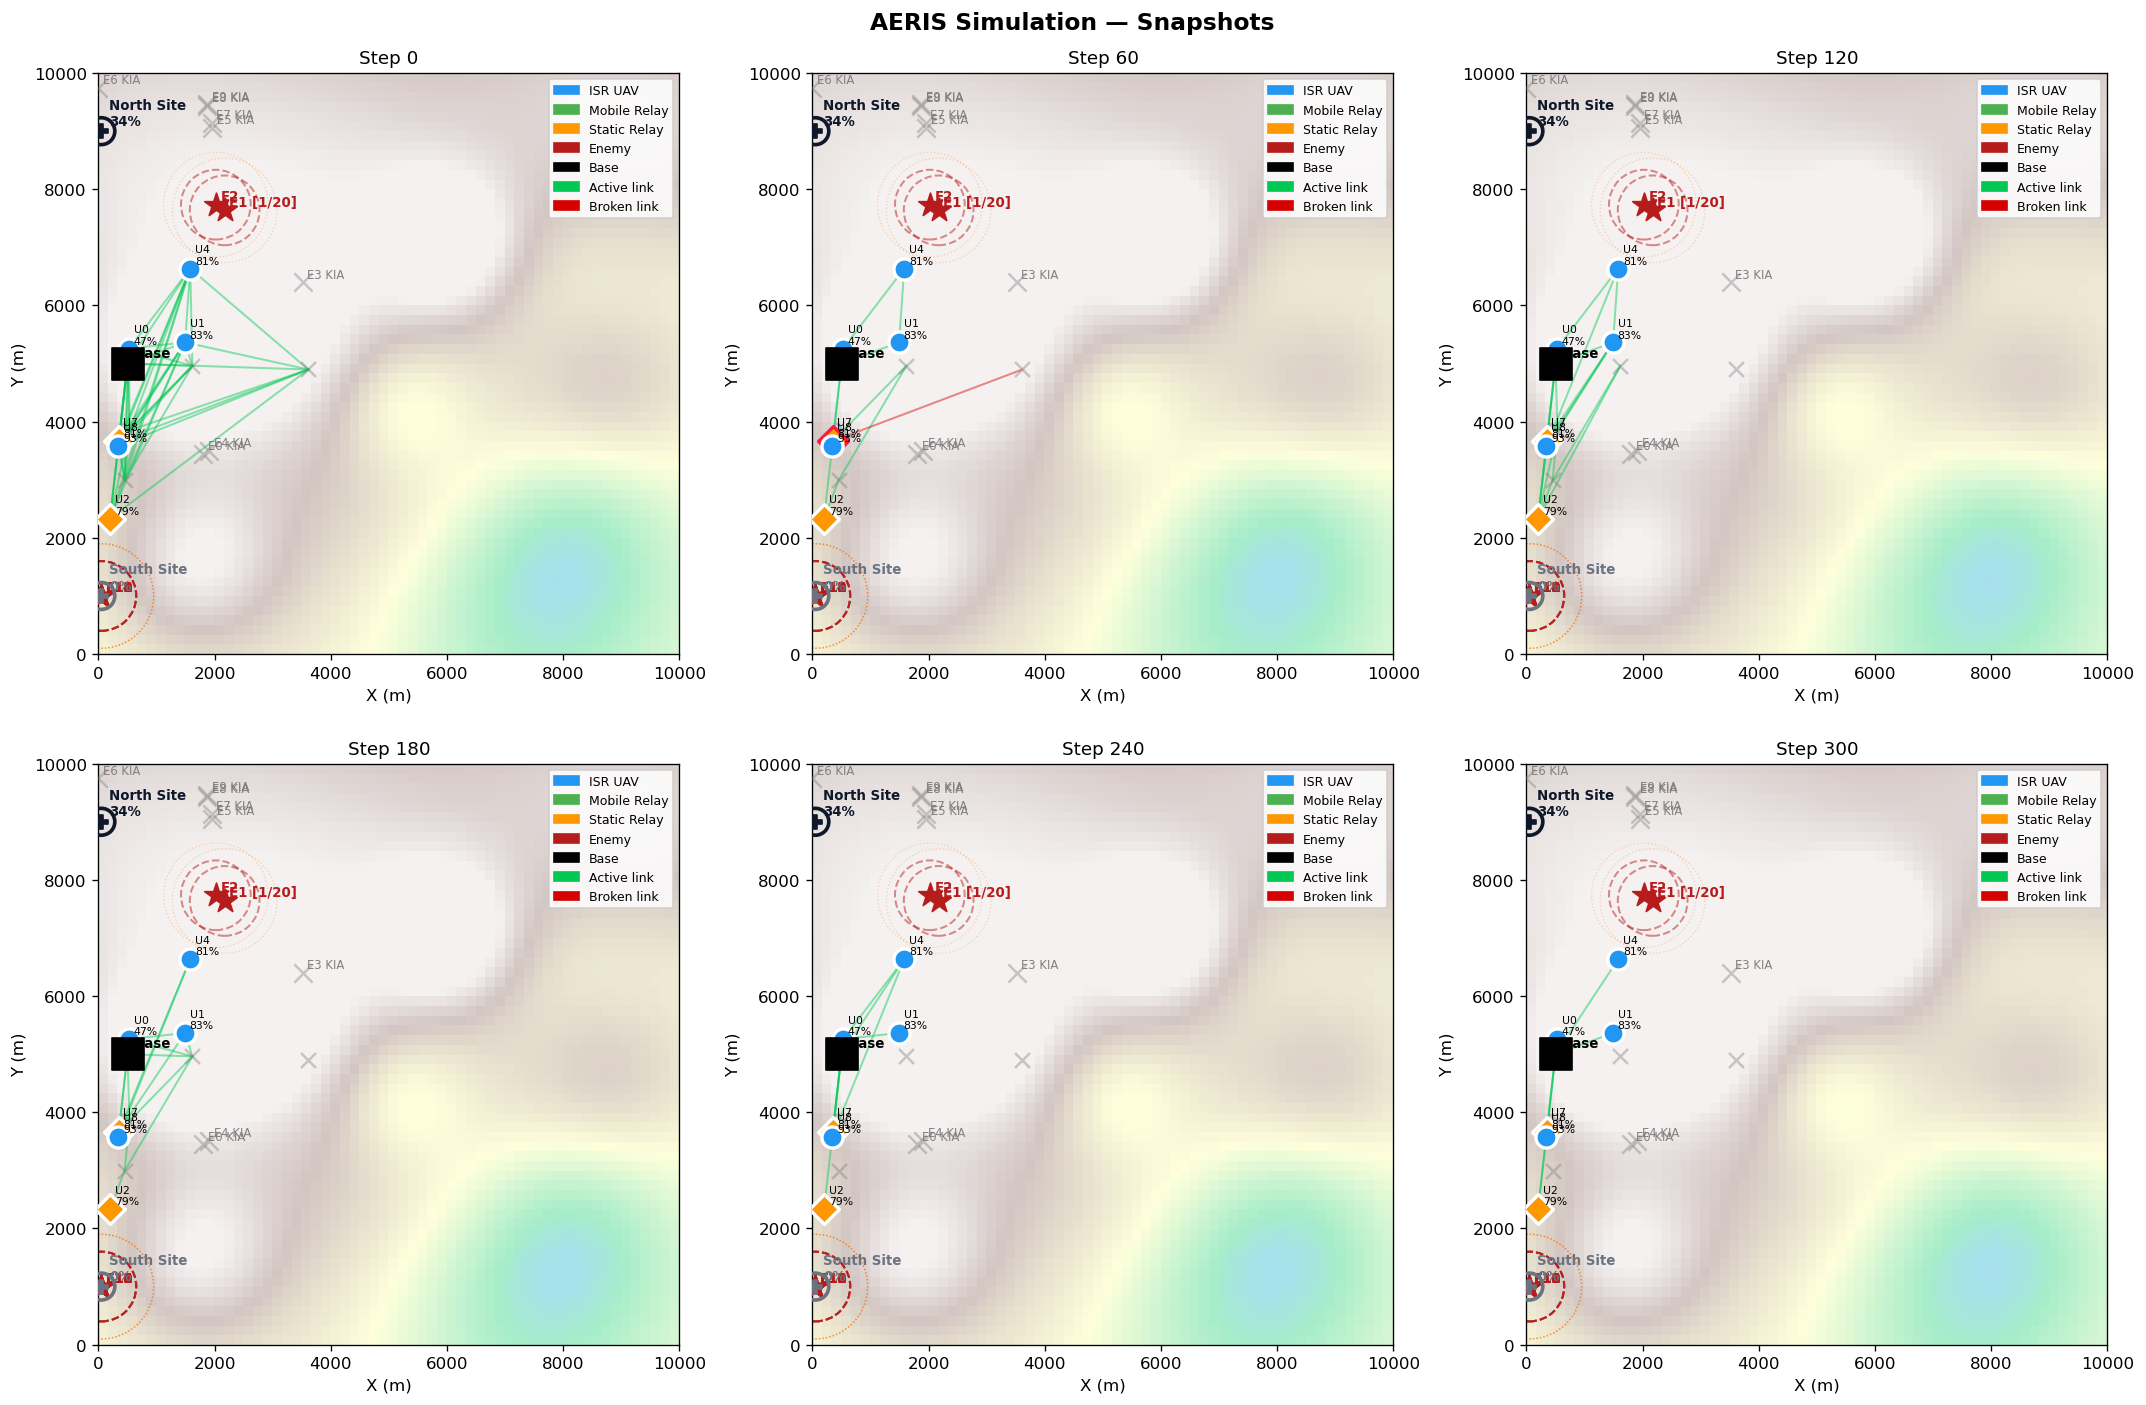
\includegraphics[width=0.92\textwidth]{aeris_dual_objective_snapshots.png}
    \caption{Dual-objective scenario snapshots. The north and south objectives
    force the UAV team to address multi-axis threats rather than only building a
    single relay chain toward the center.}
    \label{fig:dual_objective_snapshots}
\end{figure*}

\subsection{Adaptive Branching Relay Chain}
The optimizer has been extended to form multiple relay branches. Enemies are
clustered by north, center, and south bands, and relay waypoints are allocated
across active bands. This is still heuristic, but it is an important
proof-of-concept: the UAV team can adapt its communication structure to the
geometry of the threat.

\subsection{Multi-Seed Benchmarking}
A benchmark runner now evaluates policies over multiple random seeds and
produces summary statistics and banded plots. This prevents the project from
depending on a single lucky animation and allows policy variants to be compared
more honestly.

\begin{figure*}[t]
    \centering
    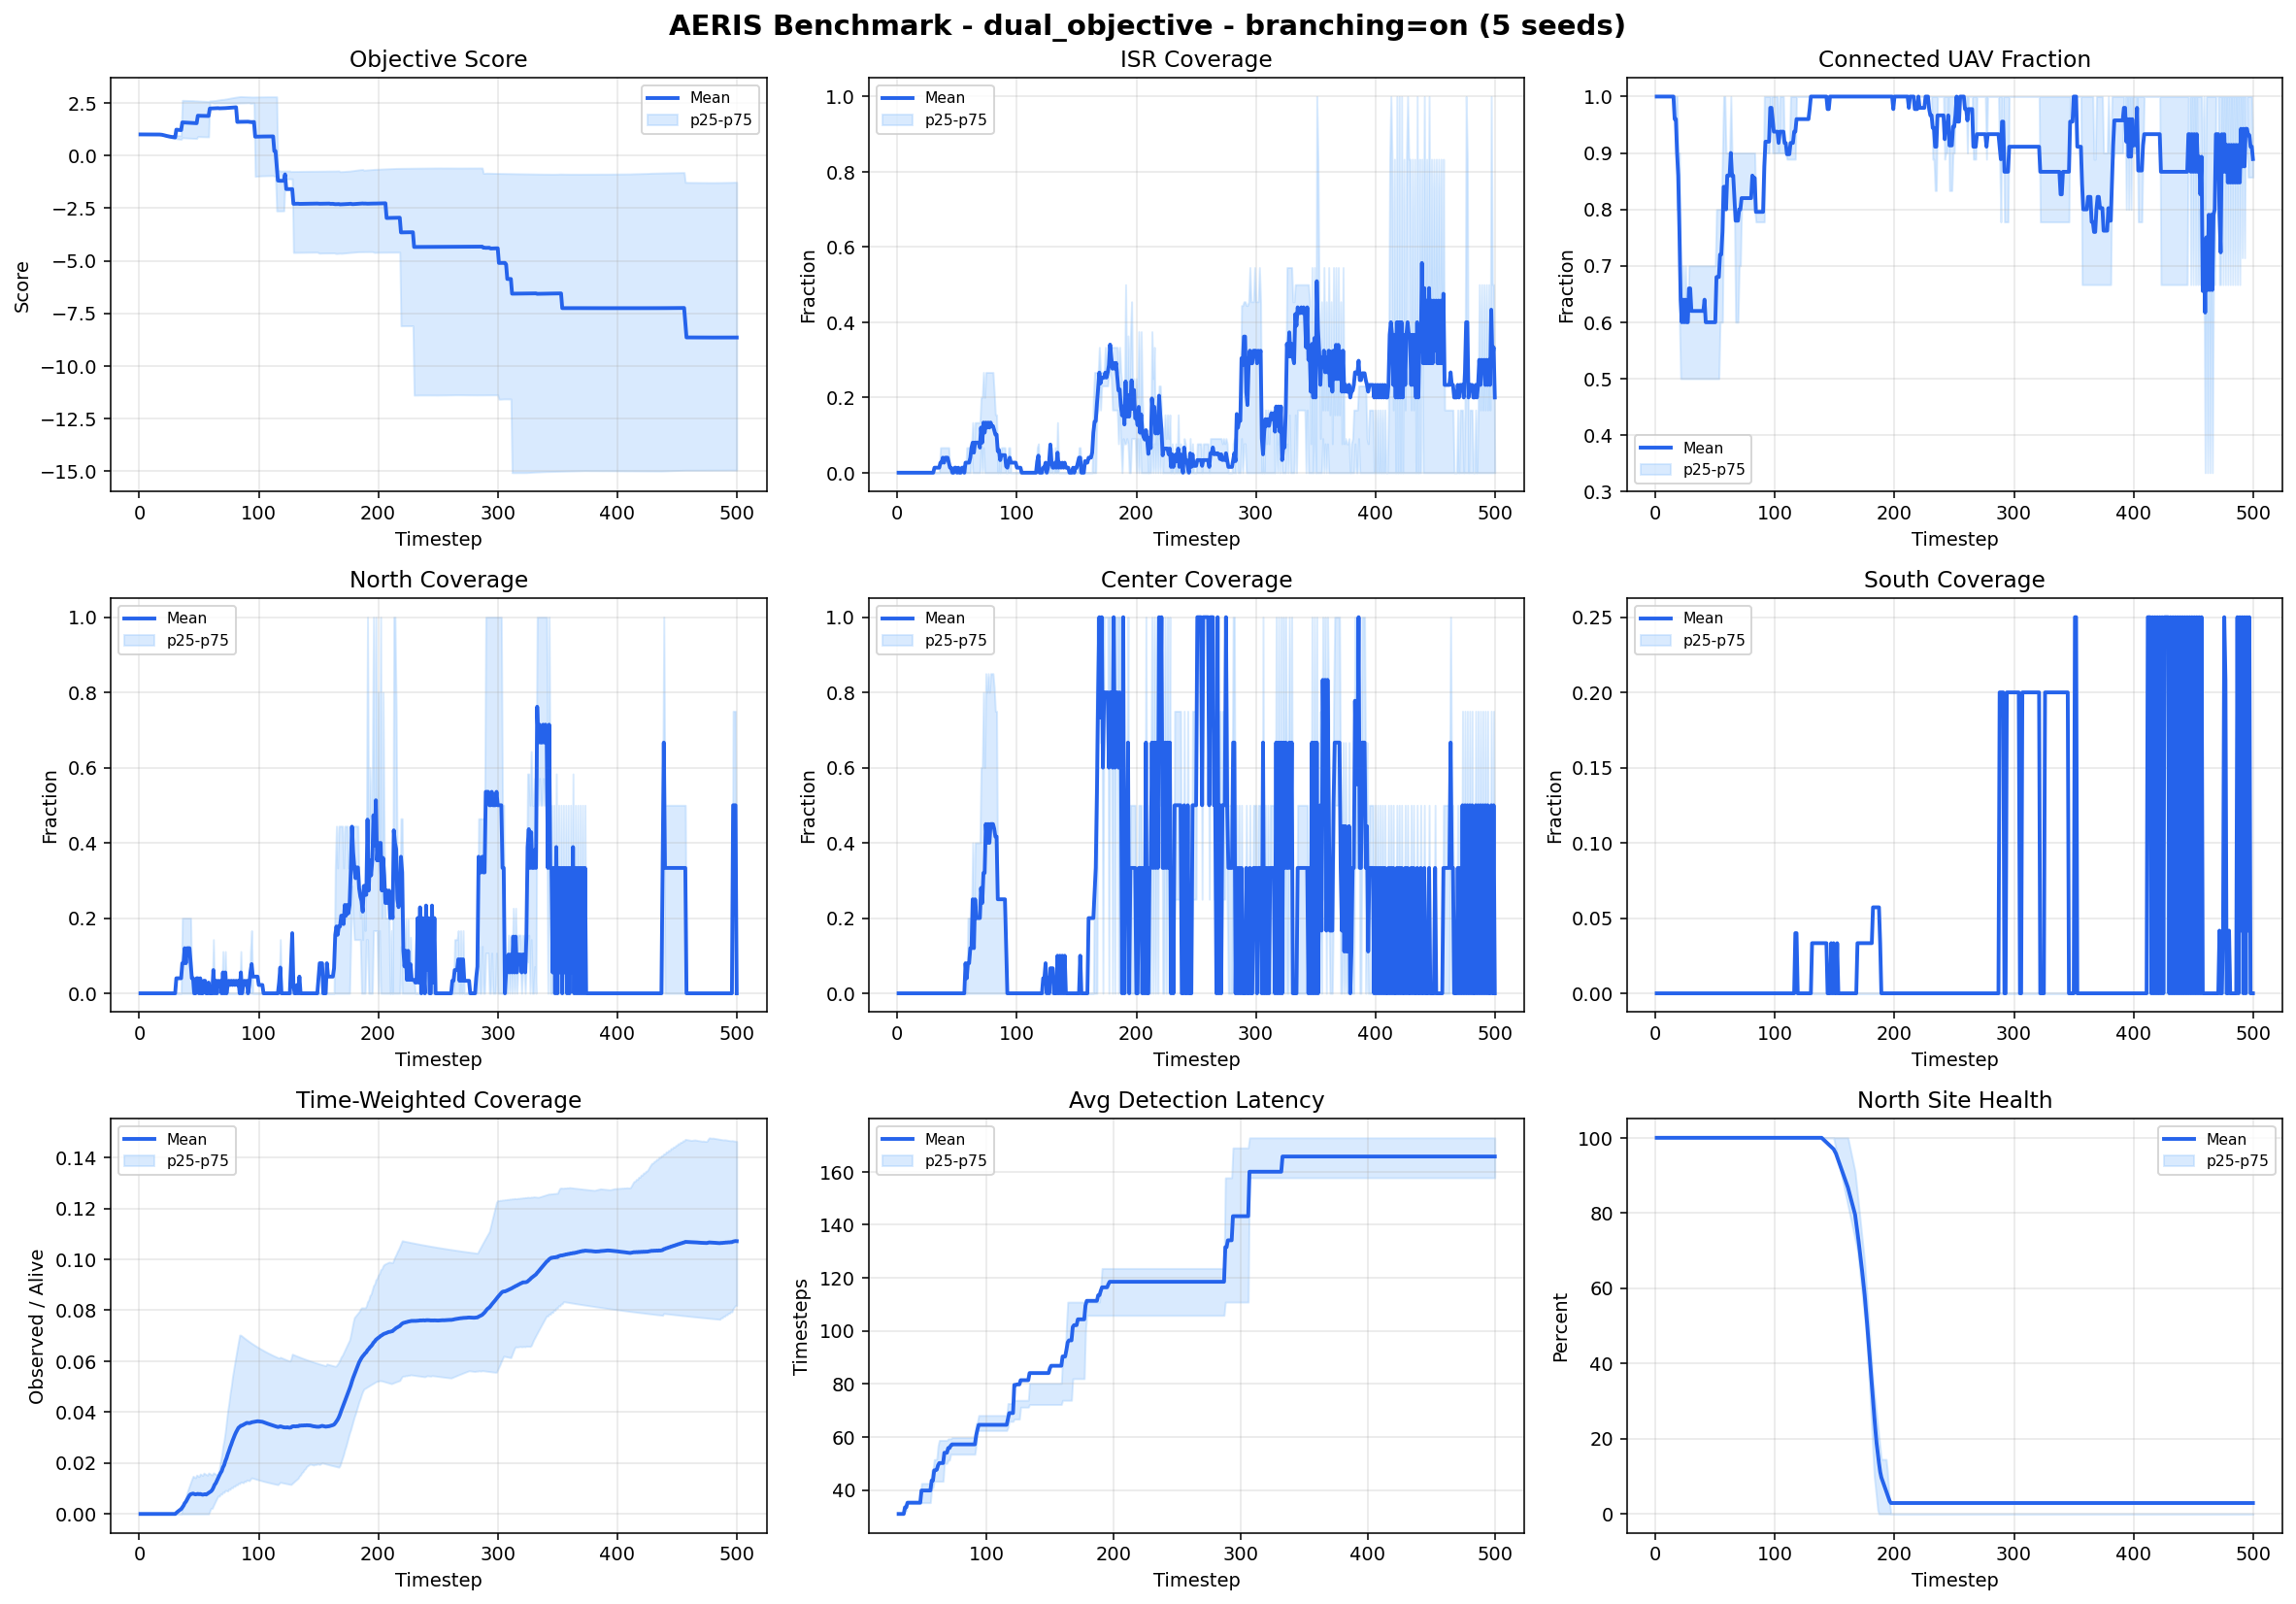
\includegraphics[width=0.92\textwidth]{benchmark_dual_on_5seed.png}
    \caption{Five-seed benchmark for the current adaptive branching controller.
    The banded plots show variability across random seeds and make policy
    comparison more statistically meaningful.}
    \label{fig:benchmark_branching}
\end{figure*}

\section{Current Optimizer Status}
The current controller should be described as a \textbf{greedy heuristic
optimizer}. It uses optimization principles, but it does not yet solve a formal
optimization problem over a planning horizon.

At each timestep, the current controller performs local decisions such as:
\begin{itemize}
    \item allocate a relay budget based on the number of available UAVs,
    \item cluster enemies into north, center, and south bands,
    \item assign relay waypoints toward active threat clusters,
    \item promote nearby ISR UAVs into relay roles when relay coverage is insufficient,
    \item assign connected ISR UAVs to nearby enemies,
    \item bias branches toward urgent objective-bound enemies.
\end{itemize}

This produces meaningful autonomous behavior and demonstrates the feasibility
of the proposed architecture. However, it is still greedy: the policy generally
chooses the best immediate role or waypoint based on local rules. It does not
yet compare multiple future action sequences, solve a constrained assignment
problem, or explicitly optimize over predicted objective damage.

\section{Experimental Findings}

\subsection{What Works}
The current greedy controller successfully demonstrates:
\begin{itemize}
    \item autonomous UAV mode switching,
    \item relay-supported connected ISR,
    \item adaptive branching in response to north and south threats,
    \item multi-seed performance evaluation,
    \item diagnostic scoring beyond visual success.
\end{itemize}

\subsection{Current Limitation}
The most important failure mode is that the north and south secondary objectives
often reach zero health. The current controller can eventually detect and strike
enemies, but it often does not prioritize objective-bound threats early enough.
This means the demo now exposes a real optimization challenge: the UAV team must
choose between relay building, broad coverage, emergency intercept, and battery
preservation under time pressure.

\subsection{Persistent ISR Watch Experiment}
A persistent ISR watch policy was tested as an attempted improvement. The idea
was to station ISR UAVs near enemy-to-objective lanes. In benchmark runs, this
performed worse than the default greedy branching policy because UAVs loitered
too passively and did not maintain decisive connected observation of urgent
enemies.

\begin{figure*}[t]
    \centering
    \begin{subfigure}{0.48\textwidth}
        \centering
        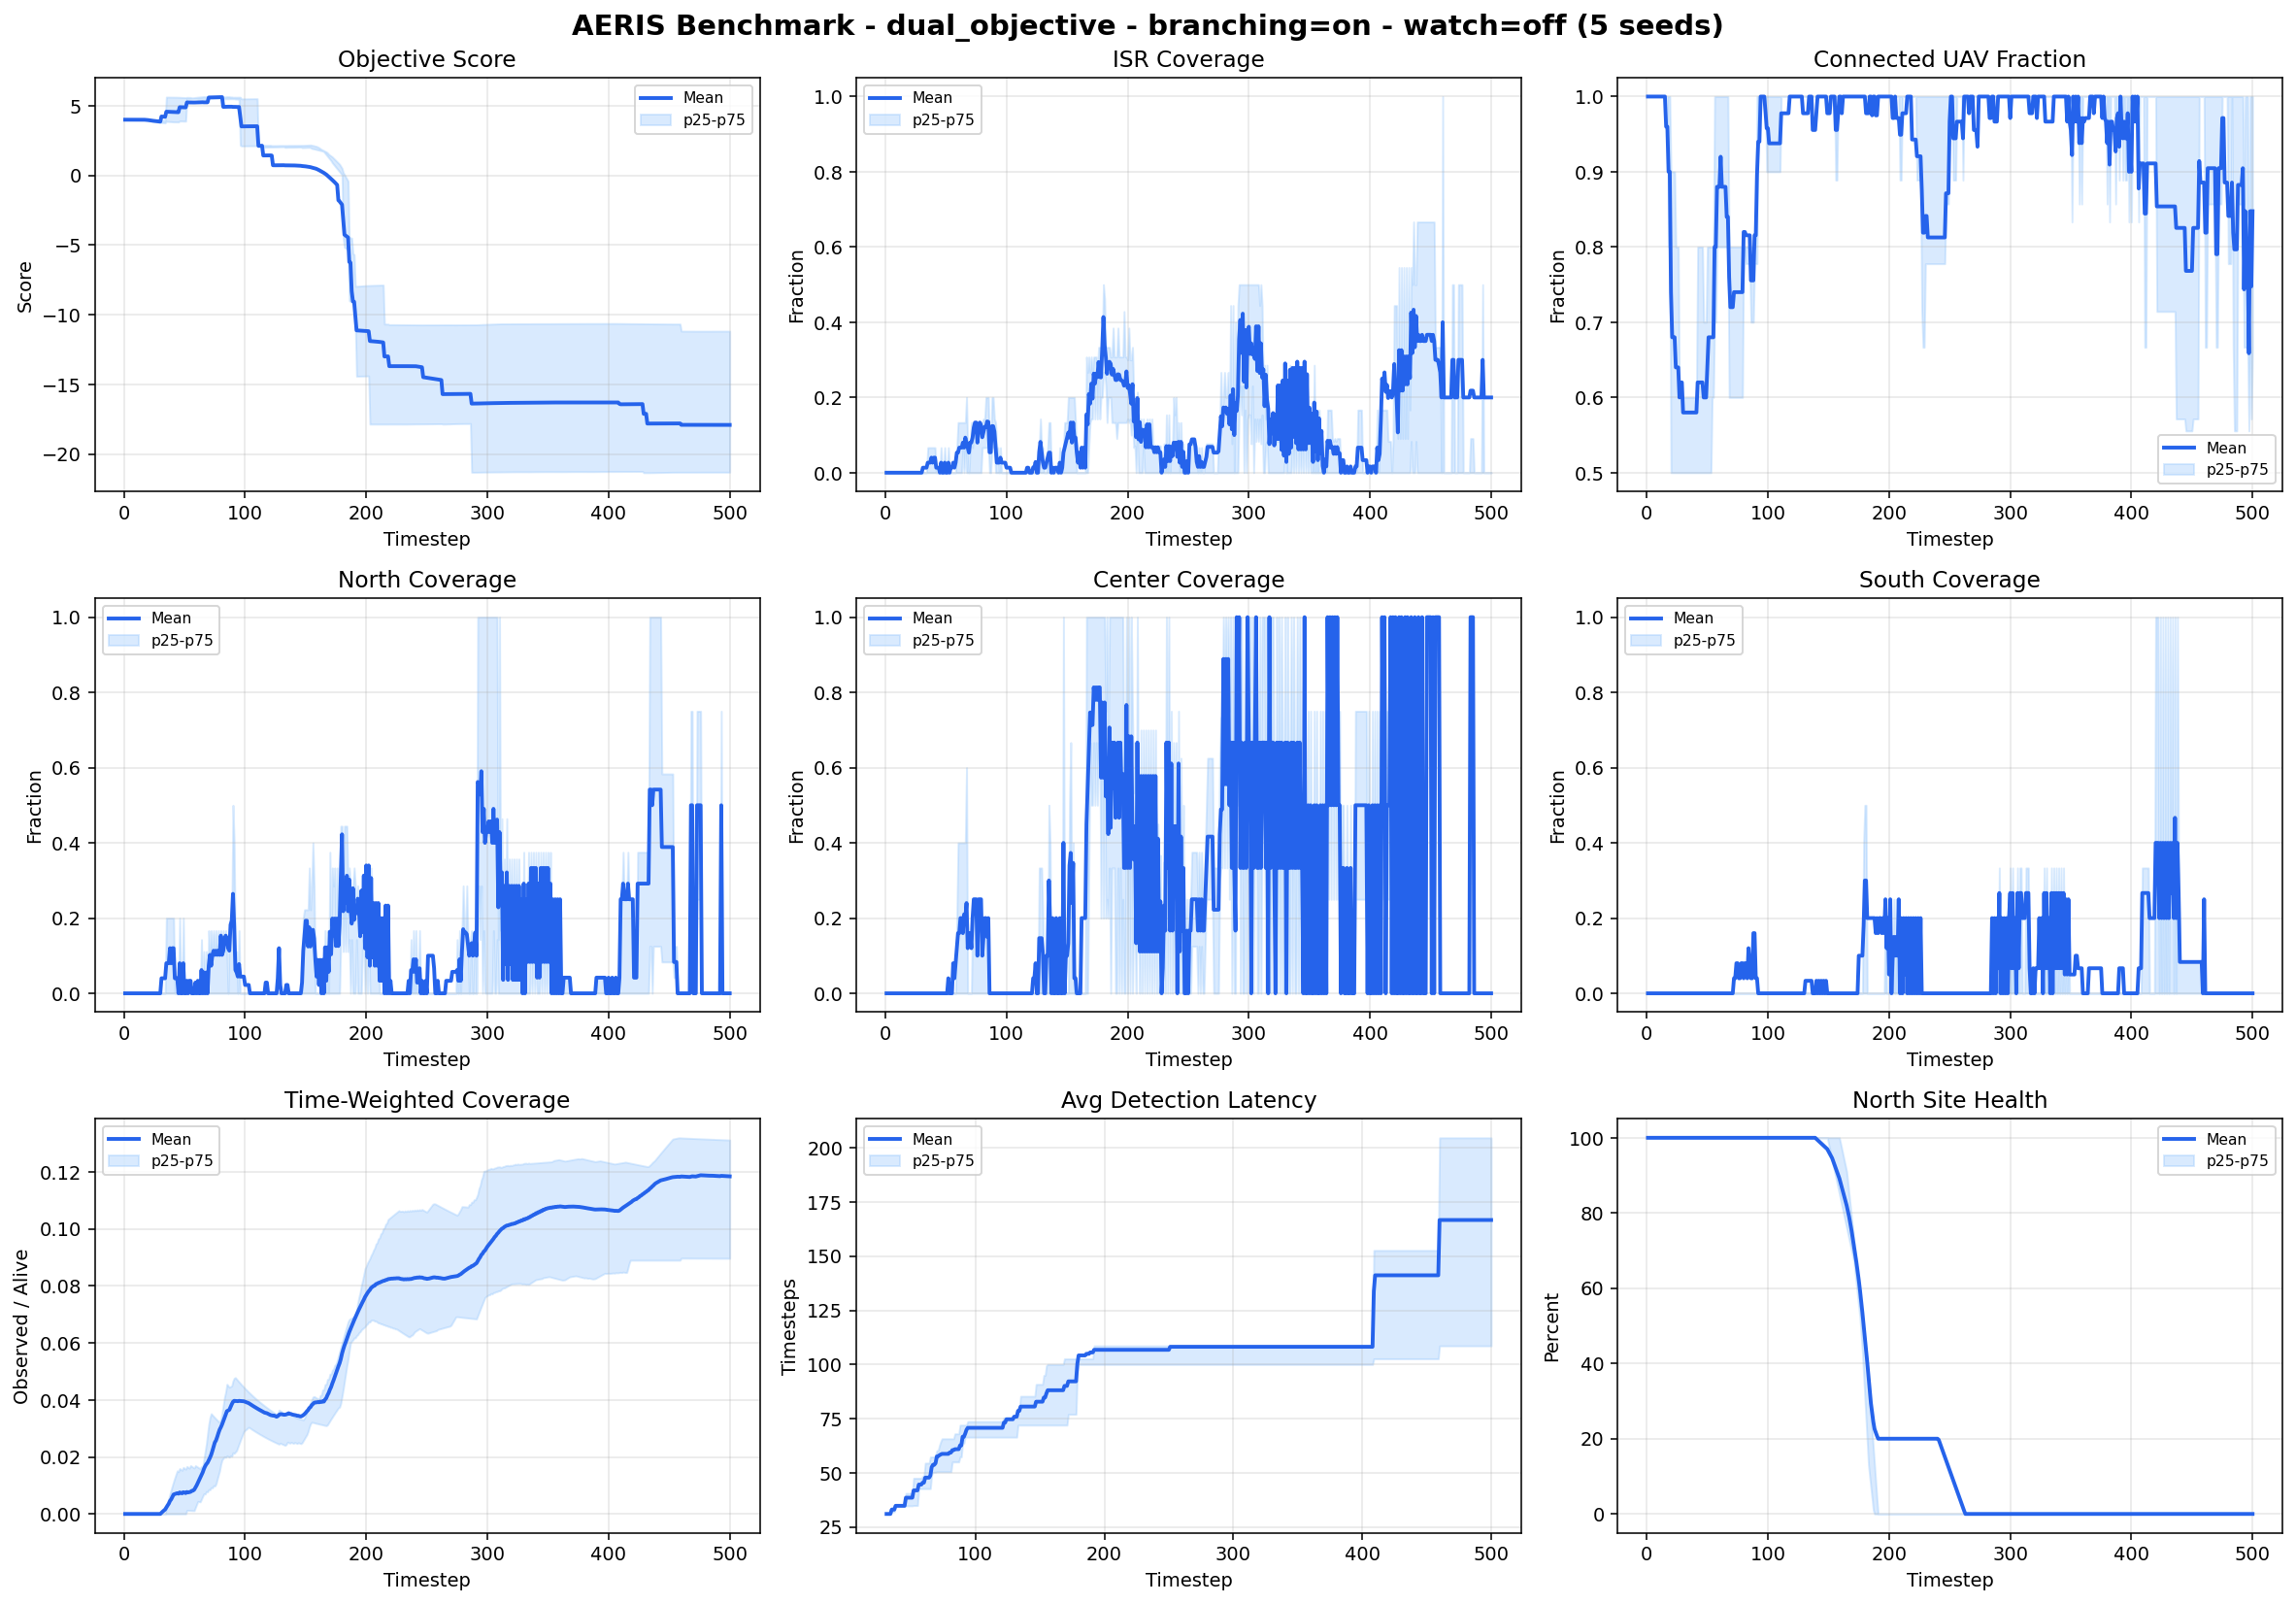
\includegraphics[width=\linewidth]{benchmark_watch_off_5seed.png}
        \caption{Persistent watch disabled.}
    \end{subfigure}
    \hfill
    \begin{subfigure}{0.48\textwidth}
        \centering
        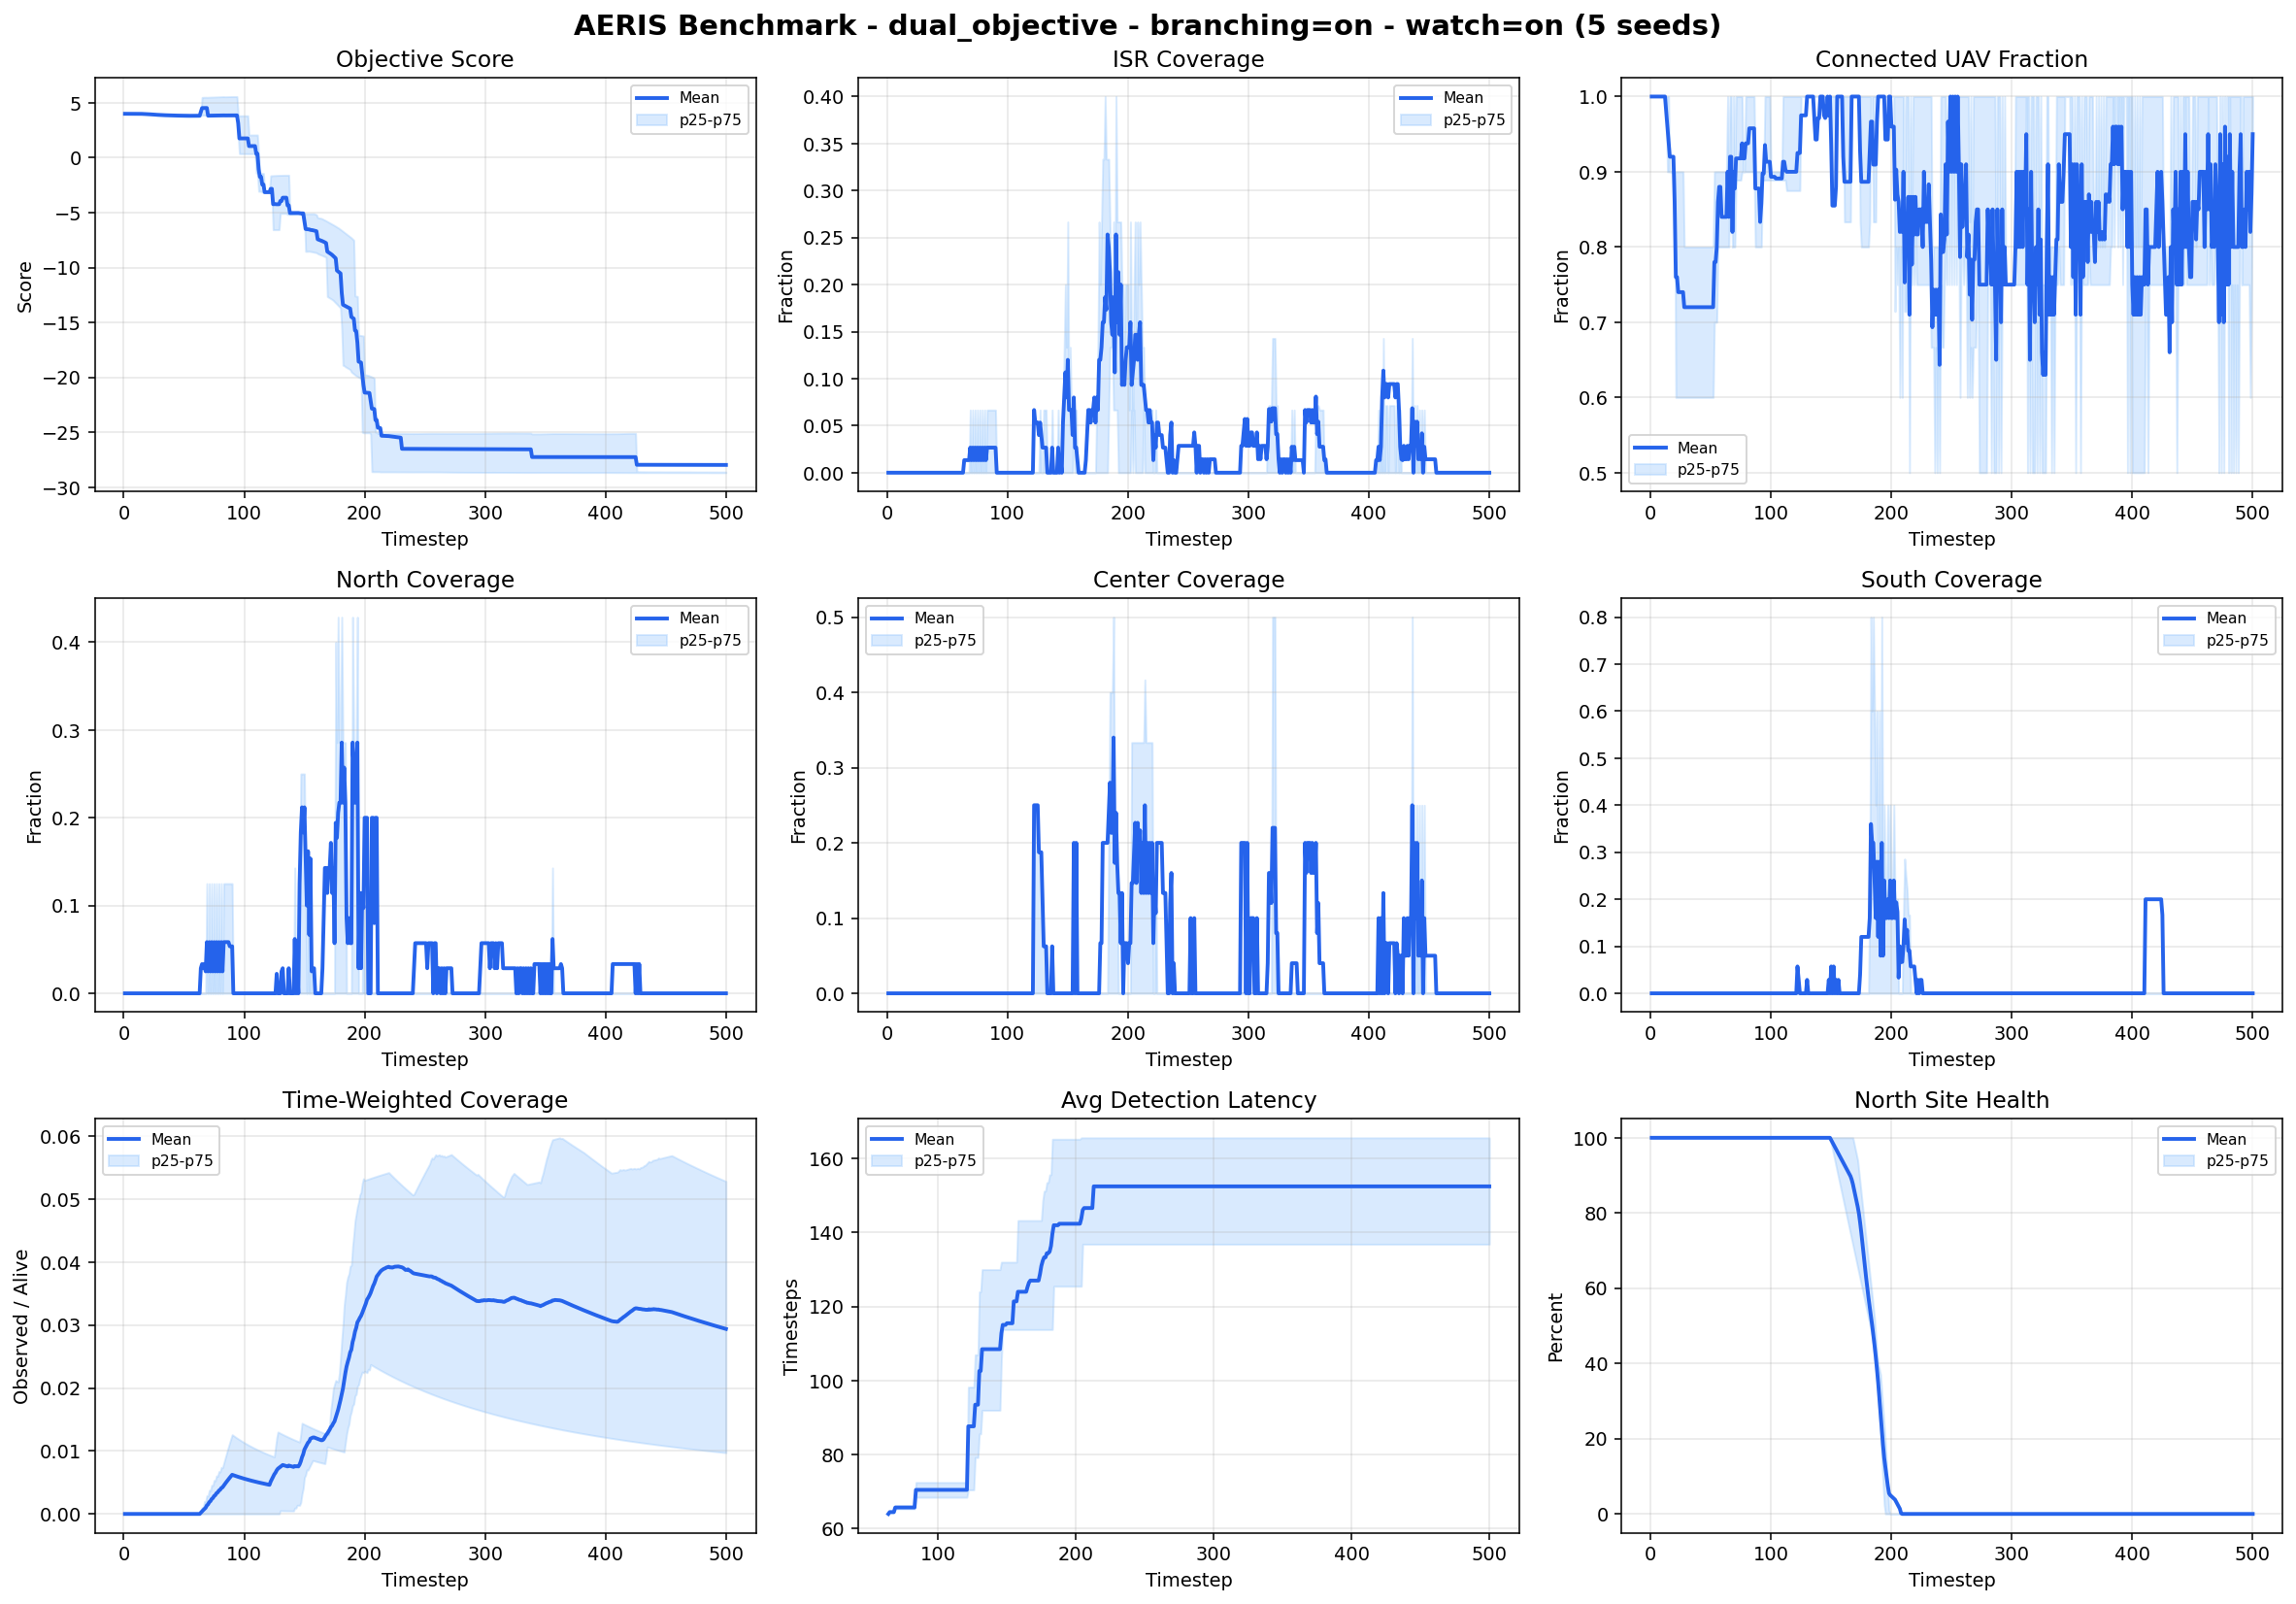
\includegraphics[width=\linewidth]{benchmark_watch_guarded_on_5seed.png}
        \caption{Persistent watch enabled.}
    \end{subfigure}
    \caption{Persistent ISR watch was evaluated and rejected as the default
    behavior. This negative result is useful because it motivates a more formal
    optimization layer rather than additional hand-tuned heuristics.}
    \label{fig:persistent_watch}
\end{figure*}

\begin{table}[t]
    \centering
    \caption{Five-seed comparison of persistent ISR watch.}
    \label{tab:watch_results}
    \begin{tabular}{lcc}
        \toprule
        Metric & Watch Off & Watch On \\
        \midrule
        Final objective & -17.90 & -27.97 \\
        Total strikes & 9.40 & 0.20 \\
        UAVs alive & 7.00 & 4.20 \\
        Enemies remaining & 5.60 & 14.80 \\
        North site health & 0.00 & 0.00 \\
        South site health & 0.00 & 0.00 \\
        \bottomrule
    \end{tabular}
\end{table}

\section{Optimization Direction for Final Project}
The final project phase will move from a greedy heuristic optimizer toward a
more explicit optimization algorithm. The planned approach is a
\textbf{finite-horizon discrete optimizer}, also known as a receding-horizon or
model-predictive controller at the high-level decision layer.

\subsection{Candidate Policy Optimization}
Instead of committing to one hand-coded behavior, the optimizer will generate a
small set of candidate policies at each decision point:
\begin{itemize}
    \item maintain current branching behavior,
    \item prioritize north objective intercept,
    \item prioritize south objective intercept,
    \item split ISR across north and south threats,
    \item prioritize relay repair,
    \item prioritize finishing already-detected enemies.
\end{itemize}

Each candidate will be rolled forward over a short horizon $H$, and the
candidate with the highest predicted mission score will be selected. Only the
first action will be executed before replanning.

\subsection{Proposed Optimization Objective}
The finite-horizon optimizer will maximize a score of the form:
\begin{equation}
\begin{aligned}
J = &\;\alpha C_{\text{ISR}}
+ \beta C_{\text{conn}}
+ \gamma H_{\text{obj}}
+ \eta S_{\text{strike}} \\
&- \lambda D_{\text{obj}}
- \mu L_{\text{detect}}
- \rho L_{\text{UAV}}
- \psi E_{\text{battery}},
\end{aligned}
\end{equation}
where $H_{\text{obj}}$ rewards remaining objective health, $D_{\text{obj}}$
penalizes predicted objective damage, $L_{\text{detect}}$ penalizes detection
latency, and $L_{\text{UAV}}$ penalizes UAV losses.

This objective connects the project more directly to multiobjective and
constrained optimization. Connectivity can be treated either as a hard
constraint or as a large penalty when ISR observations are disconnected.

\subsection{Emergency Intercept Mode}
The first optimization-driven behavior will be emergency intercept. When an
enemy is projected to reach an objective before normal coverage can suppress it,
the optimizer will prioritize assigning a connected ISR UAV to that enemy and
maintaining observation until a strike occurs. This directly addresses the
observed failure mode in the dual-objective scenario.

\subsection{Assignment Optimization}
If time allows, the project will also replace greedy UAV-to-enemy matching with
a small assignment optimization. A cost matrix can score each UAV-target pair
using distance, battery, connectivity risk, enemy urgency, and expected
objective damage. The assignment can first be solved greedily, then upgraded to
a Hungarian-style assignment if the implementation timeline allows.

\section{Two-Week Completion Plan}

\subsection{Week 1}
\begin{itemize}
    \item Formalize the finite-horizon objective function.
    \item Implement candidate policy rollout for a small set of high-level actions.
    \item Add emergency intercept as the first optimized candidate policy.
    \item Log the selected candidate policy over time for visualization.
\end{itemize}

\subsection{Week 2}
\begin{itemize}
    \item Benchmark the greedy controller against the finite-horizon optimizer.
    \item Generate final animations, snapshots, and metric plots.
    \item Update the report with the optimization formulation and results.
    \item Prepare final presentation figures showing improvement over the current heuristic.
\end{itemize}

\section{Expected Final Contribution}
The final project will present AERIS as a progression from proof-of-concept to
optimization-driven autonomy. The current greedy heuristic controller shows that
UAVs can self-organize into ISR and relay roles, maintain connected sensing, and
adapt to multi-axis threats. The final controller will make this more rigorous
by selecting actions through finite-horizon optimization. The intended final
result is a clear comparison showing that the optimization-based controller
improves objective survival, detection latency, and mission score relative to
the current greedy baseline.

\section{Conclusion}
AERIS has reached a functioning proof-of-concept stage. The simulator now
implements graph connectivity, valid ISR coverage, UAV role switching,
branching relay behavior, dual-objective threats, and multi-seed benchmarking.
The current optimizer is deliberately simple and should be described as a
greedy heuristic optimizer. This is sufficient for demonstrating the concept,
but the final project should emphasize the next step: a robust finite-horizon
optimization controller that evaluates candidate UAV assignments and relay
strategies before acting. This will align the implementation more directly with
the optimization principles in the original proposal.

\end{document}
